\documentclass[12pt,onecolumn]{article}


\usepackage{float}
\usepackage{mathtools}
\usepackage[russian]{babel}
\everymath{\displaystyle}
\usepackage{verbatim}
\usepackage[usenames]{color}
\usepackage{colortbl}

\usepackage{geometry}
\geometry{
  a4paper,
  top=15mm, 
  right=10mm, 
  bottom=15mm, 
  left=10mm
}

\begin{document}

\begin{center}
    Федеральное государственное автономное образовательное учреждение высшего образования\\
	«Национальный исследовательский университет ИТМО»
\end{center}
\vspace{1cm}


\begin{center}
    \large \textbf{Лабораторная работа №4}\\
    по дисциплине\\
    «ПРОГРАММИРОВАНИЕ»\\
	\vspace{1cm}
    Вариант №31180000,5\\
\end{center}

\vspace{10cm}
\begin{flushright}
  Выполнил студент  группы P3118: \\
  \textbf{Кокорин Всеволод Вячеславович}\\
  Преподаватель: \\
  \textbf{Письмак Алексей Евгеньевич}\\
\end{flushright}

\vspace{5cm}
\begin{center}
    г. Санкт-Петербург\\
    2022г.
\end{center}
\newpage
\tableofcontents
\newpage
\section{Текст задания}
Рулле и Филле вскочили как встрепанные. Он хотел сказать: "Рулле, нас нет", но когда он. пугался, он всегда путал буквы в словах. Карлсон и Малыш вернулись назад и снова уселись на крыльцо, но Малышу уже не было так весело, как прежде: он думал о том, как трудно обеспечить безопасность Карлсона, особенно когда рядом живут такие типы, как Рулле и Филле. А тут еще в доме будут фрекен Бок и дядя Юлиус... ах да, он ведь совсем забыл рассказать об этом Карлсону! Но Карлсон его не слушал. Он вовсю уплетал булочки и запивал их соком из маленького голубенького стаканчика, который прежде принадлежал Малышу, -- он подарил его Карлсону три месяца тому назад на его прошлый день рождения. Карлсон держал стаканчик обеими руками, как держат маленькие дети, а когда все выпил, стал его катать по полу, тоже как это делают маленькие дети. Но он и не разбился: Карлсон очень ловко придерживал его большими пальцами ног. Дело в том, что Карлсон снял башмаки и из его драных носков в красную полоску торчали большие пальцы. 
\newpage
\section{Диаграмма классов реализованной объектной модели}
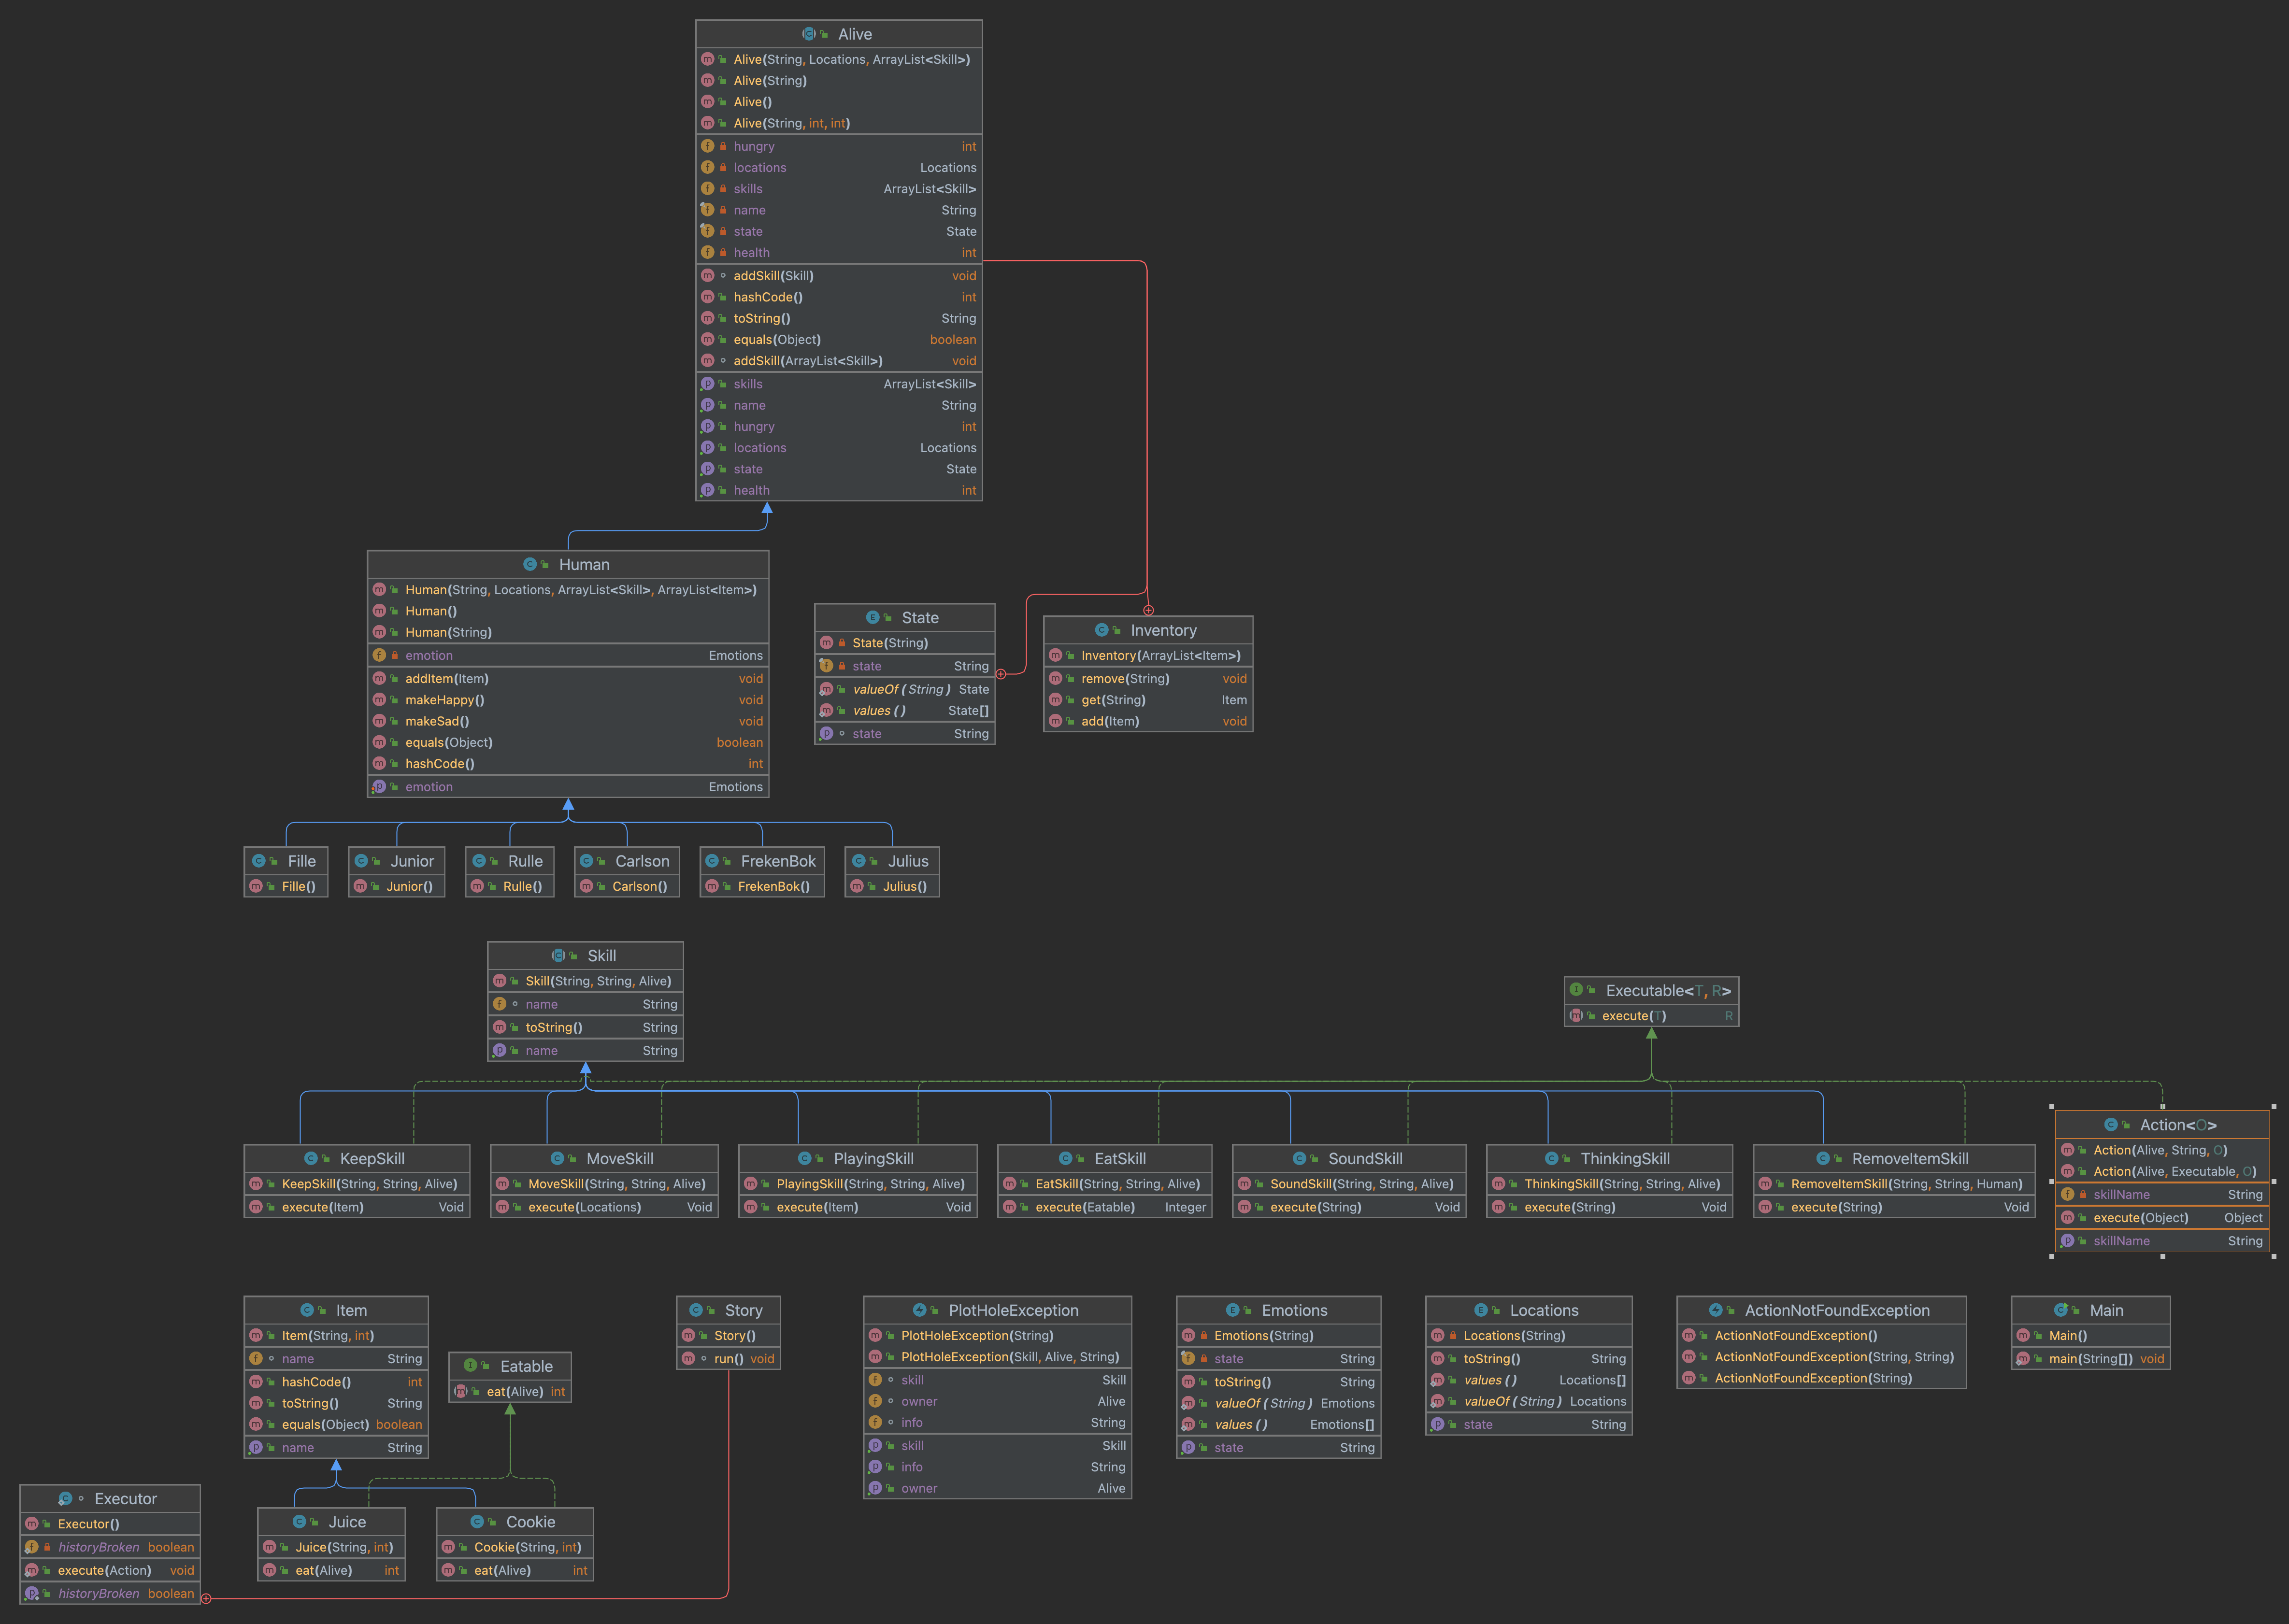
\includegraphics[width=\columnwidth]{diagram.png}
\newpage
\section{Исходный код программы}
https://github.com/Slonser/ITMO\_labs/tree/main/programming/lab4/src
\newpage
\section{Результат выполнения}
\verbatiminput{result.txt}
\newpage
\section{Вывод}
По ходу выполнения лабороторной работы я глубже ознакомился с ООП в Java, узнал про анонимные и внутренние классы.
\end{document}
